%
%  This is an example LaTeX file. The percent sign is used to mark the
% start of a comment.
%
%  - Michael Weeks, January, 2003
%
\documentclass[conference]{IEEEconf}
\usepackage[dvips]{graphics}
\usepackage{tikz}
\usepackage{dtklogos}
\usepackage[utf8]{inputenc}
\usetikzlibrary{mindmap}
\usepackage[hidelinks,pdfencoding=auto]{hyperref}
\usepackage{dirtree}
% Information boxes
\newcommand*{\info}[4][16.3]{%
  \node [ annotation, #3, scale=0.65, text width = #1em,
          inner sep = 2mm ] at (#2) {%
  \list{$\bullet$}{\topsep=0pt\itemsep=0pt\parsep=0pt
    \parskip=0pt\labelwidth=8pt\leftmargin=8pt
    \itemindent=0pt\labelsep=2pt}%
    #4
  \endlist
  };
}


\IEEEoverridecommandlockouts % Don't forget this command!

\begin{document}
  \title{Data Driven Approach For Transfer Data  From ANT+ Sensors}

  \author{{Petr Je\v{z}ek$^{1}$, Roman Mou\v{c}ek$^{1}$}
\thanks{$^{1}$Department of Computer Science and Engineering
New Technologies for the Information Society
Faculty of Applied Sciences
University of West Bohemia
Plzen, Czech Republic
        {\tt\small {jezekp, moucek}@kiv.zcu.cz}}%
\thanks{*This publication was supported by the project LO1506 of the Czech Ministry of Education, Youth and Sports}% <-this % stops a space
}
\maketitle



\begin{abstract}
Managing diseases is still more expensive in these days. For a long time people have been treated in hospotals. Fortunatelly current situation is changing also thanks to relatively cheap body sensors and raising development of systems for home treathment. It brings negligible cost saving and improves patients compfort. On the other hand it puts demands on sensors and home treatment system developers. They are depending on the efforts of data formats unification. There are standards and APIs such as Zigbee, Bluetooth low energy or ANT+ that define a protocol for data transfer. However, they do not define format for storing data from sensors in remote databases. As a solution data comming from ANT+ sensors have been studied. Then, metadata common to all sensors and raw data differing for each sensor have been defined. Next, framework for transferring data from ANT+ sensors into the proposed format implemented in NIX is described. Last, a use-case describing the transfer of data from a selected sensor into a selected neuroinformatics database is described.
\keywords{ANT+, NIX, sensor, data/metadata storage, EEGBase, data format, eHealth}
\end{abstract}

\section{Introduction}\label{sec:intro}
Managing diseases and health issues is worldwide still more expensive especially with aging population. For instance there are around 23 million people affected with heart failure \cite{bui2011epidemiology}. These people have been treated in hospitals for a long time. Nowadays, the situation is changing because relatively cheap solutions for a home treatment are coming to the market \cite{4761985, 5333913} they particularly shift patients from hospitals to their homes. It brings advantages in a better comfort for patients and it cheapens treatment itself. Home treatment systems usually use a set of sensors for monitoring of health or fitness level. Wearable sensors are usually powered from batteries. They have to operate for a long time period without possibility to change batteries frequently. That is why new protocols with the objective of low energy consumption as ZigBee \cite{Farahani:2008:ZWN:1457417}, Bluetooth Low Energy \cite{heydon2012bluetooth} or ANT \cite{zaloker2014ant} has been developed.  Data from these sensors are transfered to remote servers where they are processed and results are visualized. Sensors usually measure a large collection of body parameters. Integration of these sensors creates Body Area Networks (BAN). When the number of sensors connected to BAN is increasing requirements to the management and a long term storage and sustainability of data are also increasing.

Although low energy consumption standards for data transfer exist they are still too fragmented to enable easy manipulation with obtained data. Moreower these standards do not provide menans for a long term storage and management of data. As a solution this paper presents an approach of using a unified NIX format for encapsulating ANT+ sensor data. Then the transfer to a remote storage is also presented. 

The paper is organized as follows. Section \ref{sec:state-of-the-art} describes current approaches in the domain. Then Section \ref{sec:ant-plus-profiles} describes existing ANT+ profiles and selects most suitable profiles for eHealth domain. Section \ref{sec:framework} describes a proposed framework that facilitates the conversion of sensors data to an output NIX format. Then Section \ref{sec:use-case} demonstrates the usage of proposed transformation. Last Section \ref{sec:future-work} summarizes the current work and provide an outlook to the future.

\section{State of The Art}\label{sec:state-of-the-art}

An approach presented in \cite{mehmood2014ontology} defines three layers ontology describing data from different sensors. This ontology facilitates to programmers the development of tools for processing sensors data. A Sensor-Cloud infrastructure \cite{5635688} represents physical sensors as virtual sensors stored in a Cloud infrastructure. The Cloud manages sensors capabilities. So called Semantic Sensor Web \cite{4557983} is based on an annotation of sensors data by means of Semantic Web. Such annotated data can be distributed via the Internet.


\section{ANT+ Profiles Discussion}\label{sec:ant-plus-profiles}
ANT+ protocol is so popular because of its low energy consumption and because it provides good means to describe body parameters or fitness level. The main benefit are so called ``device profiles``.  They define sending data over the network in a consistent way \cite{innovations2013ant}. When the data transfer profiles are defined they facilitate development of sensors and also management of sensor data in application programs.

ANT+ profiles support a large scale of activities such as Cycling or Walking, or measurement of body parameters such as Heart Rate, Blood pressure, Weight, Muscle Oxygen Monitor etc. If we browse individual profiles in a detail we can observe attributes that are common for all profiles including e.g.: a device name, a device status, a manufacturer, a signal strength or a battery status. Then, there are other attributes varying for individual profiles. 

We can observe that individual profile attributes represent raw sensor data while common attributes describe metadata. 

\section{Proposed Framework}\label{sec:framework}

\subsection{Requirements}\label{sec:requirements}

Due to the absence of a format or a data structure for representing data from sensors we are designing a framework that enables collecting of sensor data and storing both raw data and metadata in defined structure. The framework have to use a widely accepted format in order to stored data can be reused in third-party systems. The format must be robust and flexible to cover a heterogeneous nature of sensor data and to provide a long term sustainability. Next, the format must be accepted by larger scientific community. 

\begin{figure*}
\centering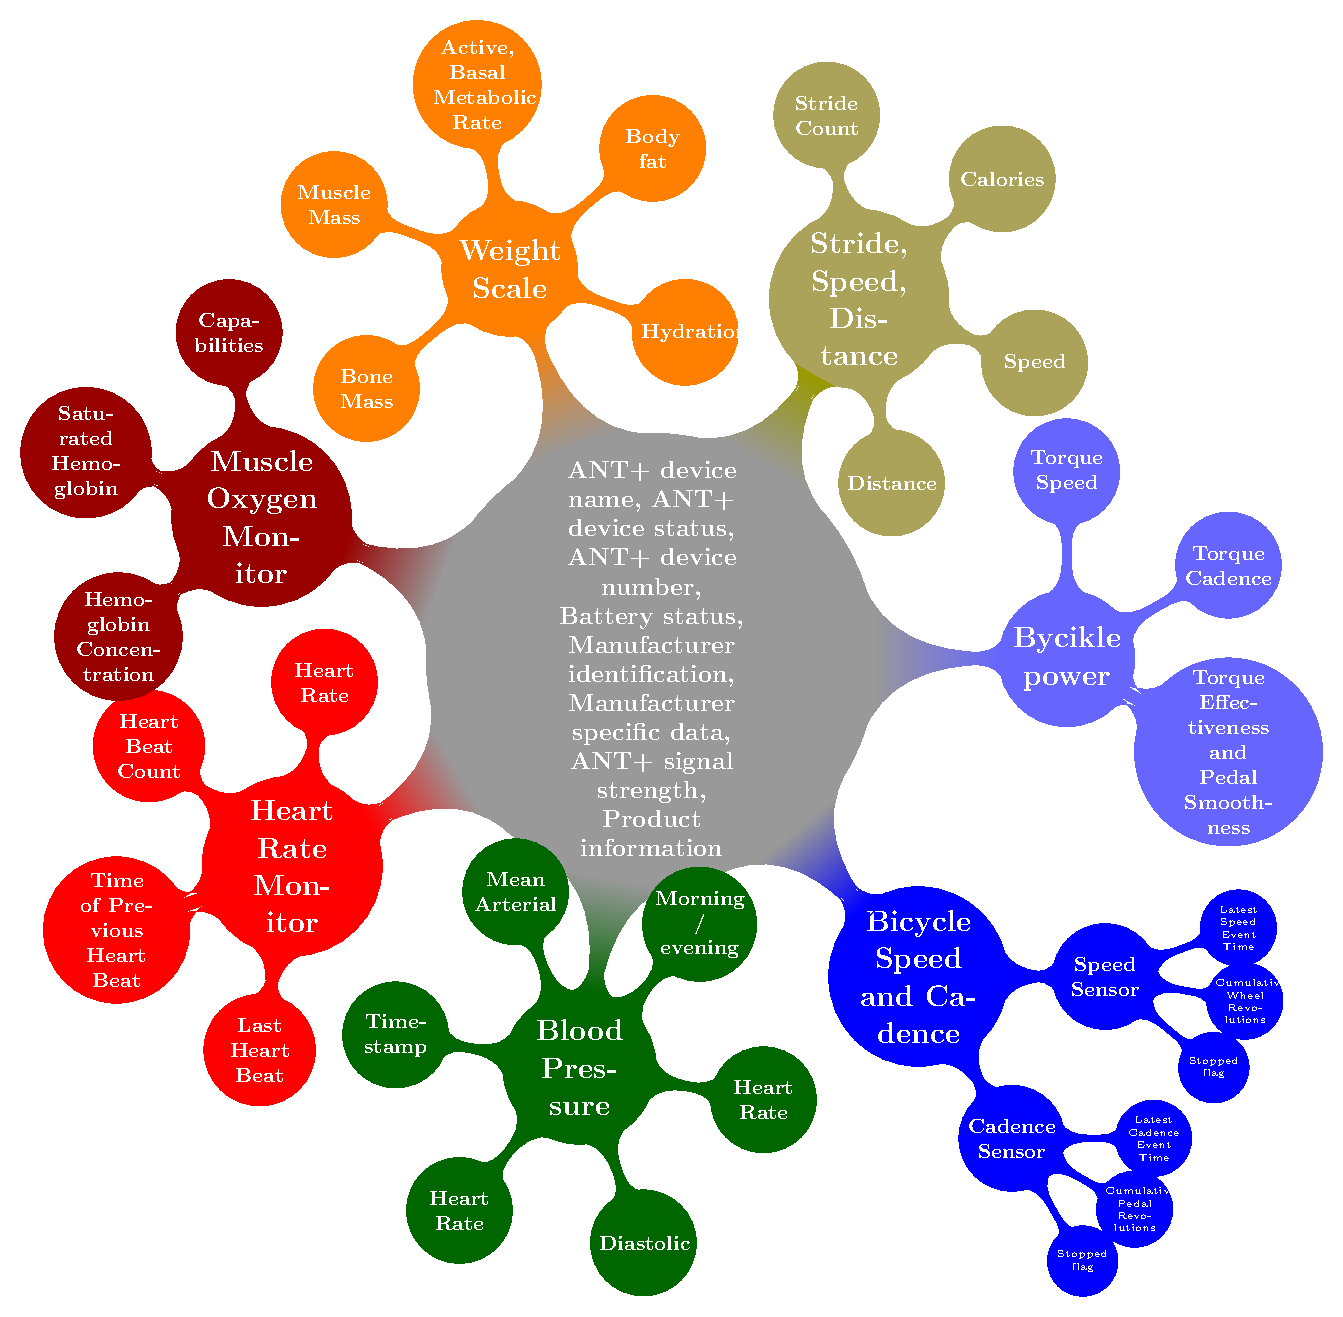
\includegraphics[width=12cm, height=10cm]{AntPlusProfiles}
\caption{\label{AntPlus}ANT+ Profiles Network}
\end{figure*}

\subsection{Format Discussion}

As a member of International Neuroinformatics Coordinating Facility (INCF) \cite{wvangeit:Bjaalie:JNeurosci:2007} we are responsible for the development of a hardware and software infrastructure for electrophysiology experiments. Within INCF we are a member of the working group of the INCF Task Force on Electrophysiology\footnote{http://www.incf.org/programs/datasharing/ electrophysiology-task-force}. There were introduced two approaches towards defining a standard. The first one uses the Hierarchical Data Format (HDF5) \cite{hdf5}. HDF5 is portable and extensible format supporting an unlimited variety of datatypes and it is designed for flexible and efficient I/O and for high volume and complex data. The second approach is OdML~\cite{10.3389/fninf.2011.00016}. It is a~free form tree-like structure of sections, properties and values. It is a suitable metadata format because of its platform-independence, simplicity, and human-readability. Moreover, it ensures a compatibility with other systems developed in neuroinformatics community, for example \cite{10.3389/conf.fninf.2014.18.00029}, \cite{10.3389/conf.fninf.2014.18.00053}, and~\cite{10.3389/conf.fninf.2013.09.00025}. A next step of the task force is merging of these two approaches\cite{10.3389/conf.fninf.2013.09.00069}. The result is the NIX format~\cite{Stoewer:2014}. It provides a data model for storing experimental data in HDF5, together with metadata in the odML format.




\subsection{Proposed Mapping}

We selected these ANT+ profiles that can be used for monitoring of person health or fitness level. We determined a common metadata from these profiles and individual raw data. Figure \ref{AntPlus} show a graphical relationship of the profiles. A middle circle shows common metadata while other circles are the selected profiles and their raw data. 

The NIX model consists of several main elements: Block, DataArray, Tag, MultiTag, Source, Group and Dimension. Each element consists several attributes such as id, name and specific attributes for individual elements. Moreover, each element can consist a link to odML metadata. We use a simplified NIX model for mapping ANT+ elements. A Source represents an ANT+ device, the DataArray represents raw data coming from the device sensor, the Dimension represents a description of axis. Last, the Block wraps complete recording.

\begin{figure}
  %\vspace{-0.2cm}
  \centering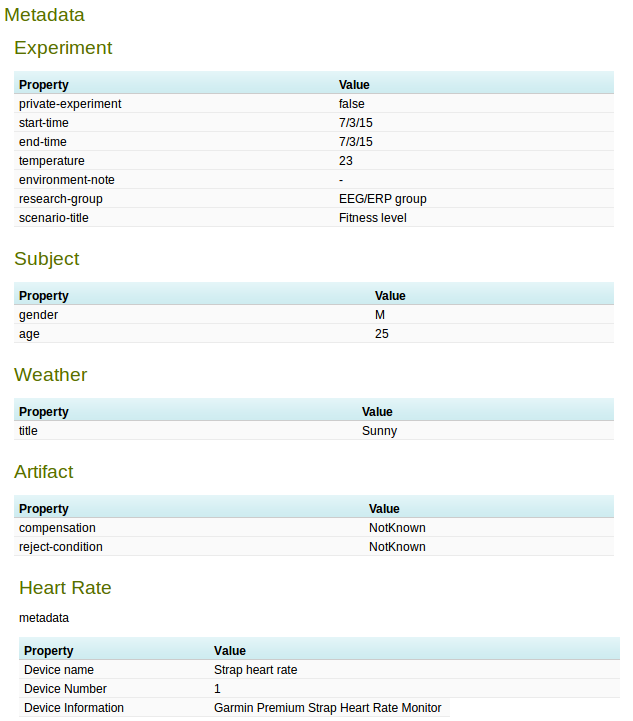
\includegraphics[width=8cm]{portal_example.png}
  \caption{Data stored in EEGBase}
  \label{fig:EEGBase}
 \end{figure}


\section{Use Case}\label{sec:use-case}

The presented framework serves mainly for designers or programmers of complete systems intended for home monitoring of end-users. Let's assume following use-case. A programmer wants to implement a system for heart rate monitoring of elderly people. This system has following requirements: It must use an easy to use sensor for a heart rate monitoring, data from this sensor must be easily transferred to a computer where they are stored and evaluated. Moreover, there can be regular medical checks where a physician can use these long term heart rate records to check a health condition of the patient or eventually set a treatment. This requires to both the patient and the doctor have access to an infrastructure that provide aims to store an manage users data. Such infrastructure must provide data security, consistency and sustainability.

As a solution so called neuroinformatics databases and approaches such as CRCNS \cite{CRCNS}, Helmholtz \cite{10.3389/conf.fninf.2013.09.00025}, Carmen \cite{fgibson:Watson2007}, INCF Dataspace \cite{dataspace} or EEGBase \cite{ISI:000306821100004} are developing. These databases are the most promising approaches. Most of them just accepted or are going to accept the NIX format as a standardized one.

There is lot of heart rate monitor straps. We use Garmin Premium Strap Heart Rate Monitor for this use-case. It is an ANT+ supported device, we use Android SDK\footnote{http://developer.android.com/sdk/} that enables reading data by Android smart phones. We integrate the SDK into a custom mobile application MoBio\footnote{https://github.com/NEUROINFORMATICS-GROUP-FAV-KIV-ZCU/MoBio} that reads data from ANT+ sensors and store them on a SD card. The user can pair available sensors, record data and visualize them. This solution is available to large scale of users because of cheap Android smart phones and heart rate monitor straps on the market.

Finally, MoBio integrates our framework that is why we can store data into a NIX file. When MoBio reads data it parses basic metadata such as device name, product information etc. Next metadata are transferred into a structure with one section and several properties as it is expressed in Figure \ref{odML}. Then heart beats are continuously read. These beats are stored into a data array. Figure \ref{NIX-ex} shows a hear beats signal stored in DataArray. The Source element has an attribute metadata that contains a link to metadata stored in the odML structure.

Once data are stored they can be transferred to a suitable neuroinformatics database. Figure \ref{fig:EEGBase} shows data stored an visualized in EEGBase. There is a complex description of an experiment containing metadata from Heart Rate strap. The raw data are stored as well.

\begin{figure}

\dirtree{%
.1 Section.
.2 name = heart\_rate.
.2 type = metadata.
.2 Properties.
.3 Device name = Strap heart rate monitor.
.3 Device number = 1.
.3 Product Information = Garmin Premium Strap Heart Rate Monitor.
}
\caption{\label{odML}odML metadata for heart rate sensor}
\end{figure}

\begin{figure*}
\centering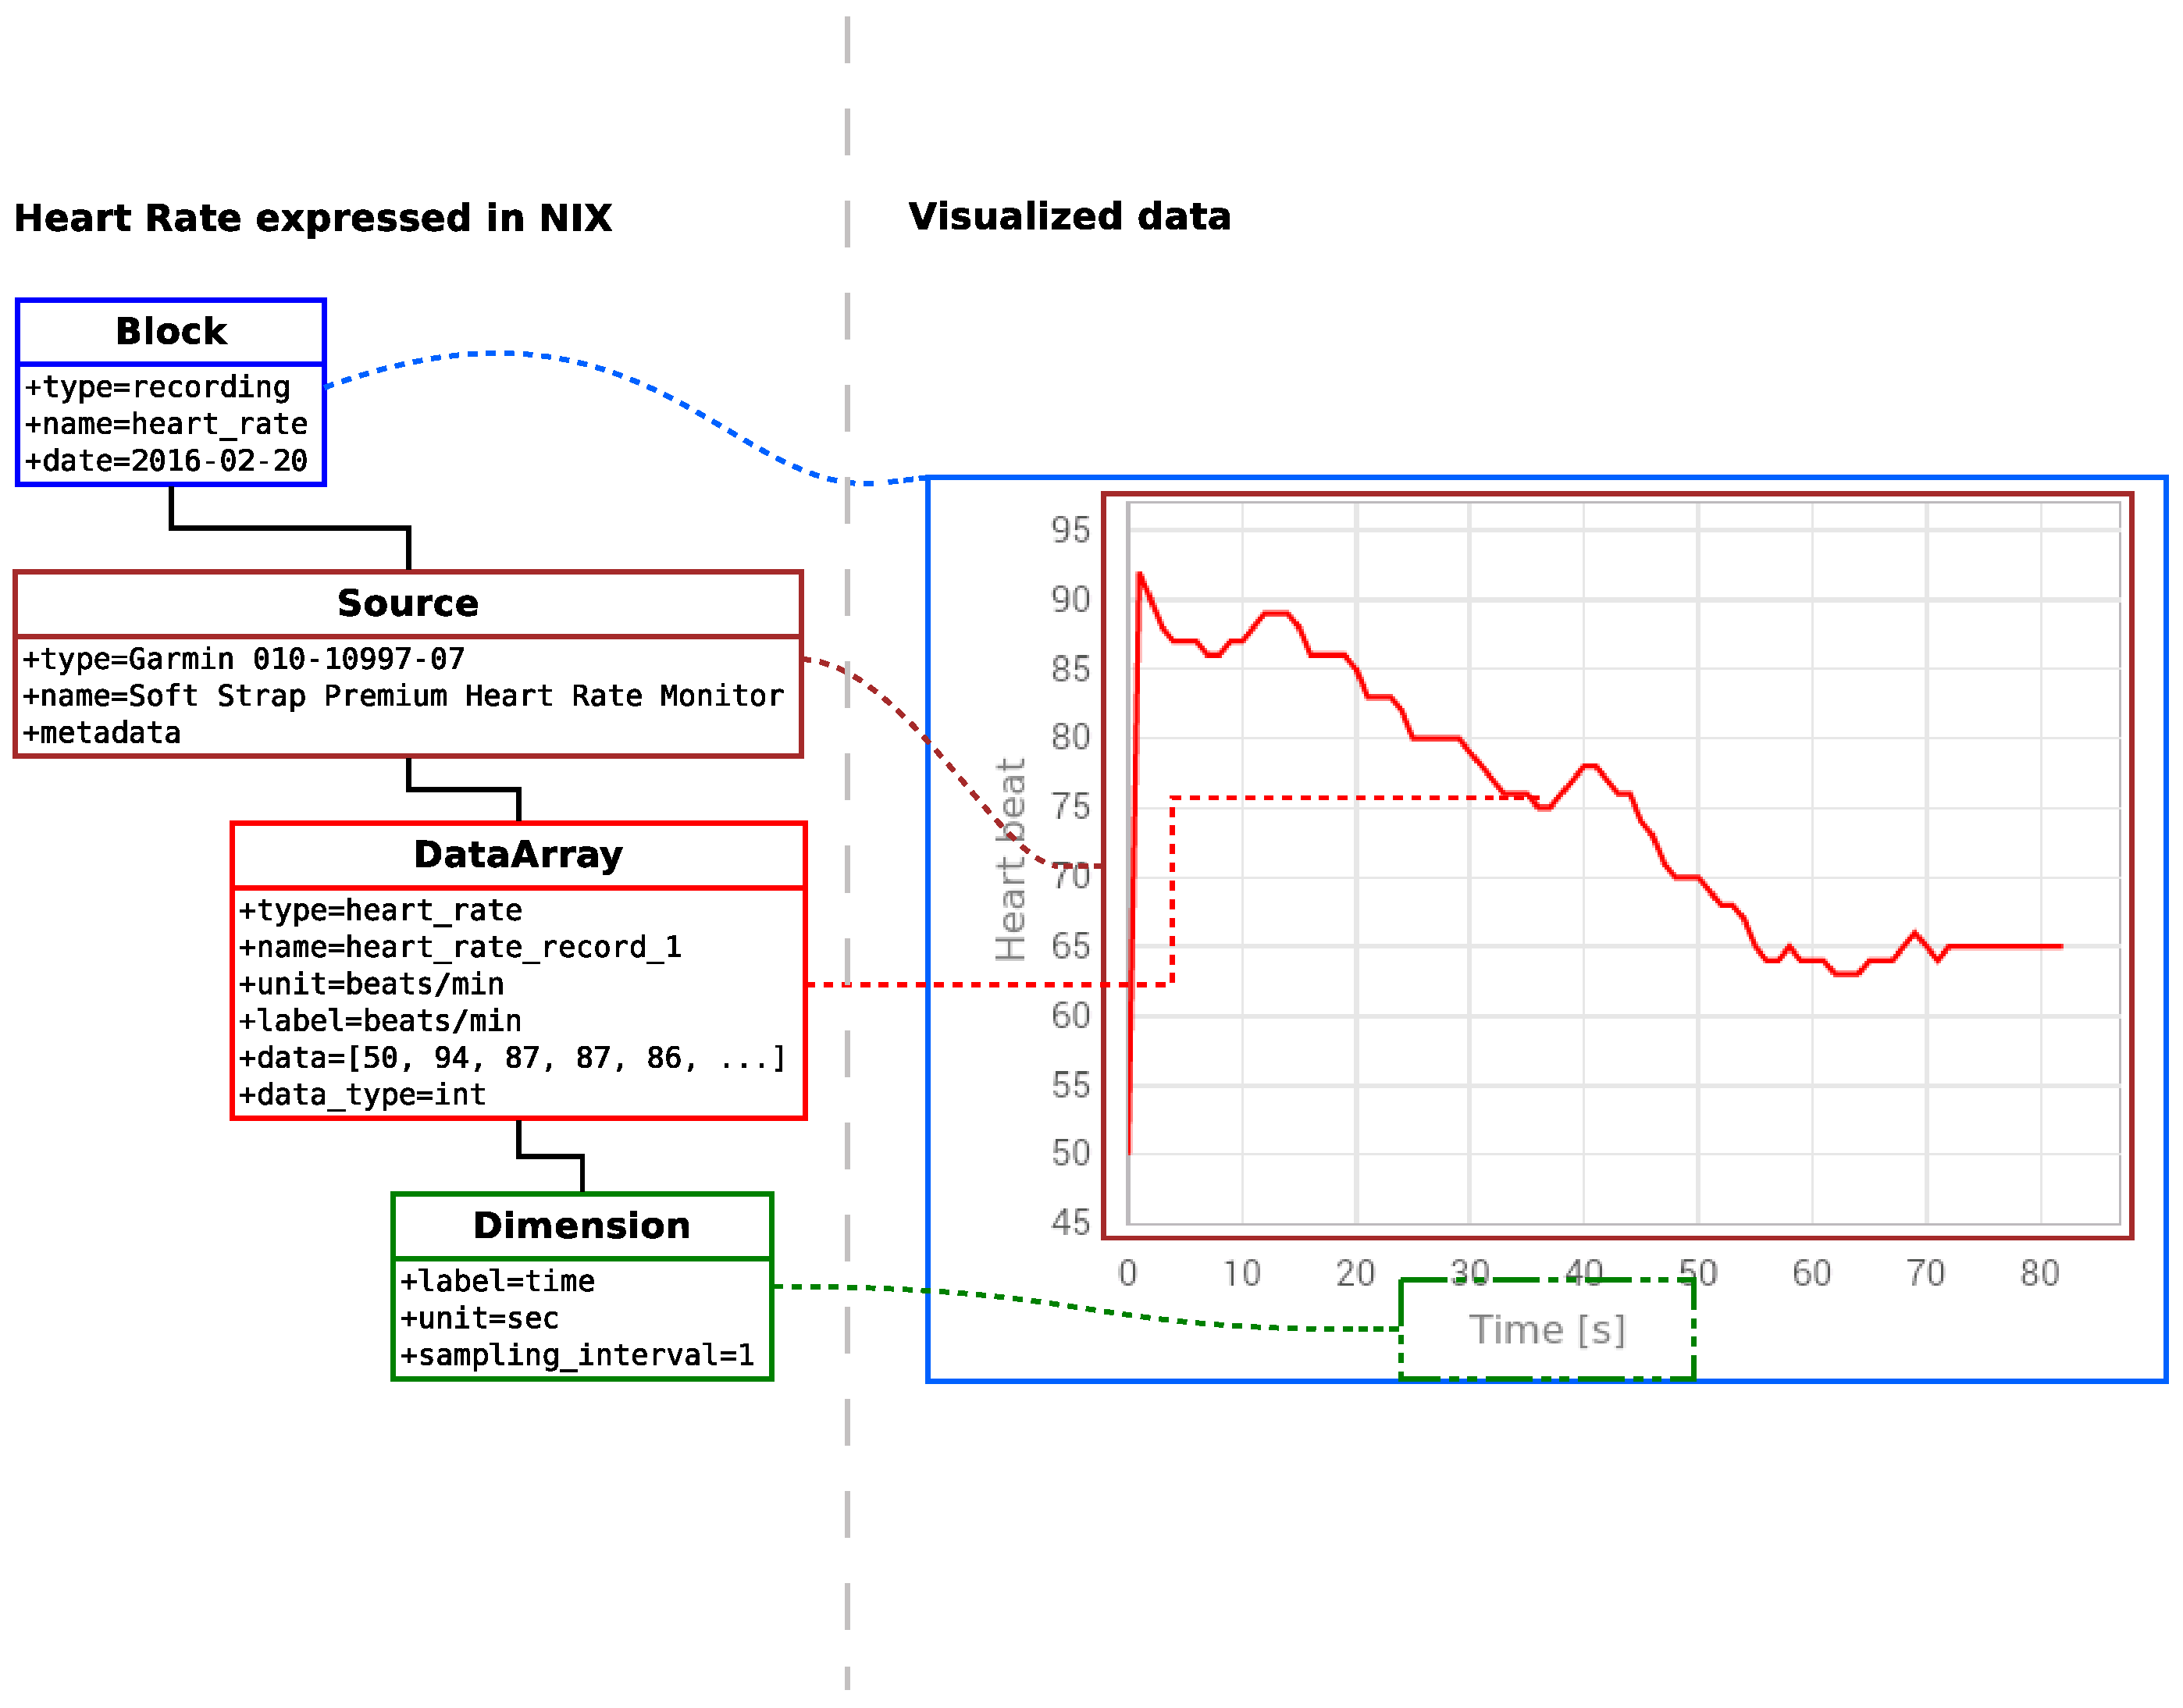
\includegraphics[width=13cm]{NIX-example}
\caption{\label{NIX-ex}Heart rate measurement transferred to NIX}
\end{figure*}



\section{Conclusions and Future Work}\label{sec:future-work}

Because of raising popularity of sensors for home treatment several low energy standards has been defined. These standards enables transffer data from body sensors into common computers where they can be processed. The one of the most often used is ANT+ supported by significant sensors producers. Although a transfer protocol is defined and several APIs for working with sensors exist there is not defined a standard for storing of sensors data. As long as home treatment systems use proprietary data formats systems could not be easily integrated with sensors. It brings serious complications for designers of such systems. In this paper we have described a framework that aim is to overcome these difficulties by designing a framework that maps data from ANT+ sensors into a widelly accepted format NIX. This format brings advantages of two layers structure. First the metadata strucuture uses a flexible format odML and the second data strucure is based on HDF5 format. The definition of this two layers has been also significant contribution of this work. Next, advantage of this solution is the support of NIX format withing community.

The functionality of the frawemork is described on a simple use case. Our future work is to test it on a large collection of sensors and test the data transfer to a larger collection of neuroinformatics database. We also plan to invite developers of home tratment systems to integrate the framework into their solutions. 

Next, when the framework is fully tested we will work on the tranformation of data from Blueetooth low energy into the NIX format as well. 



% Now here is the reference section.

\bibliographystyle{IEEEtran}
% argument is your BibTeX string definitions and bibliography database(s)
\bibliography{EMBC-2016,citations-ic4awe-2016,bibliography,neuroportals}
\end{document}